
\begin{figure}
  \centering
  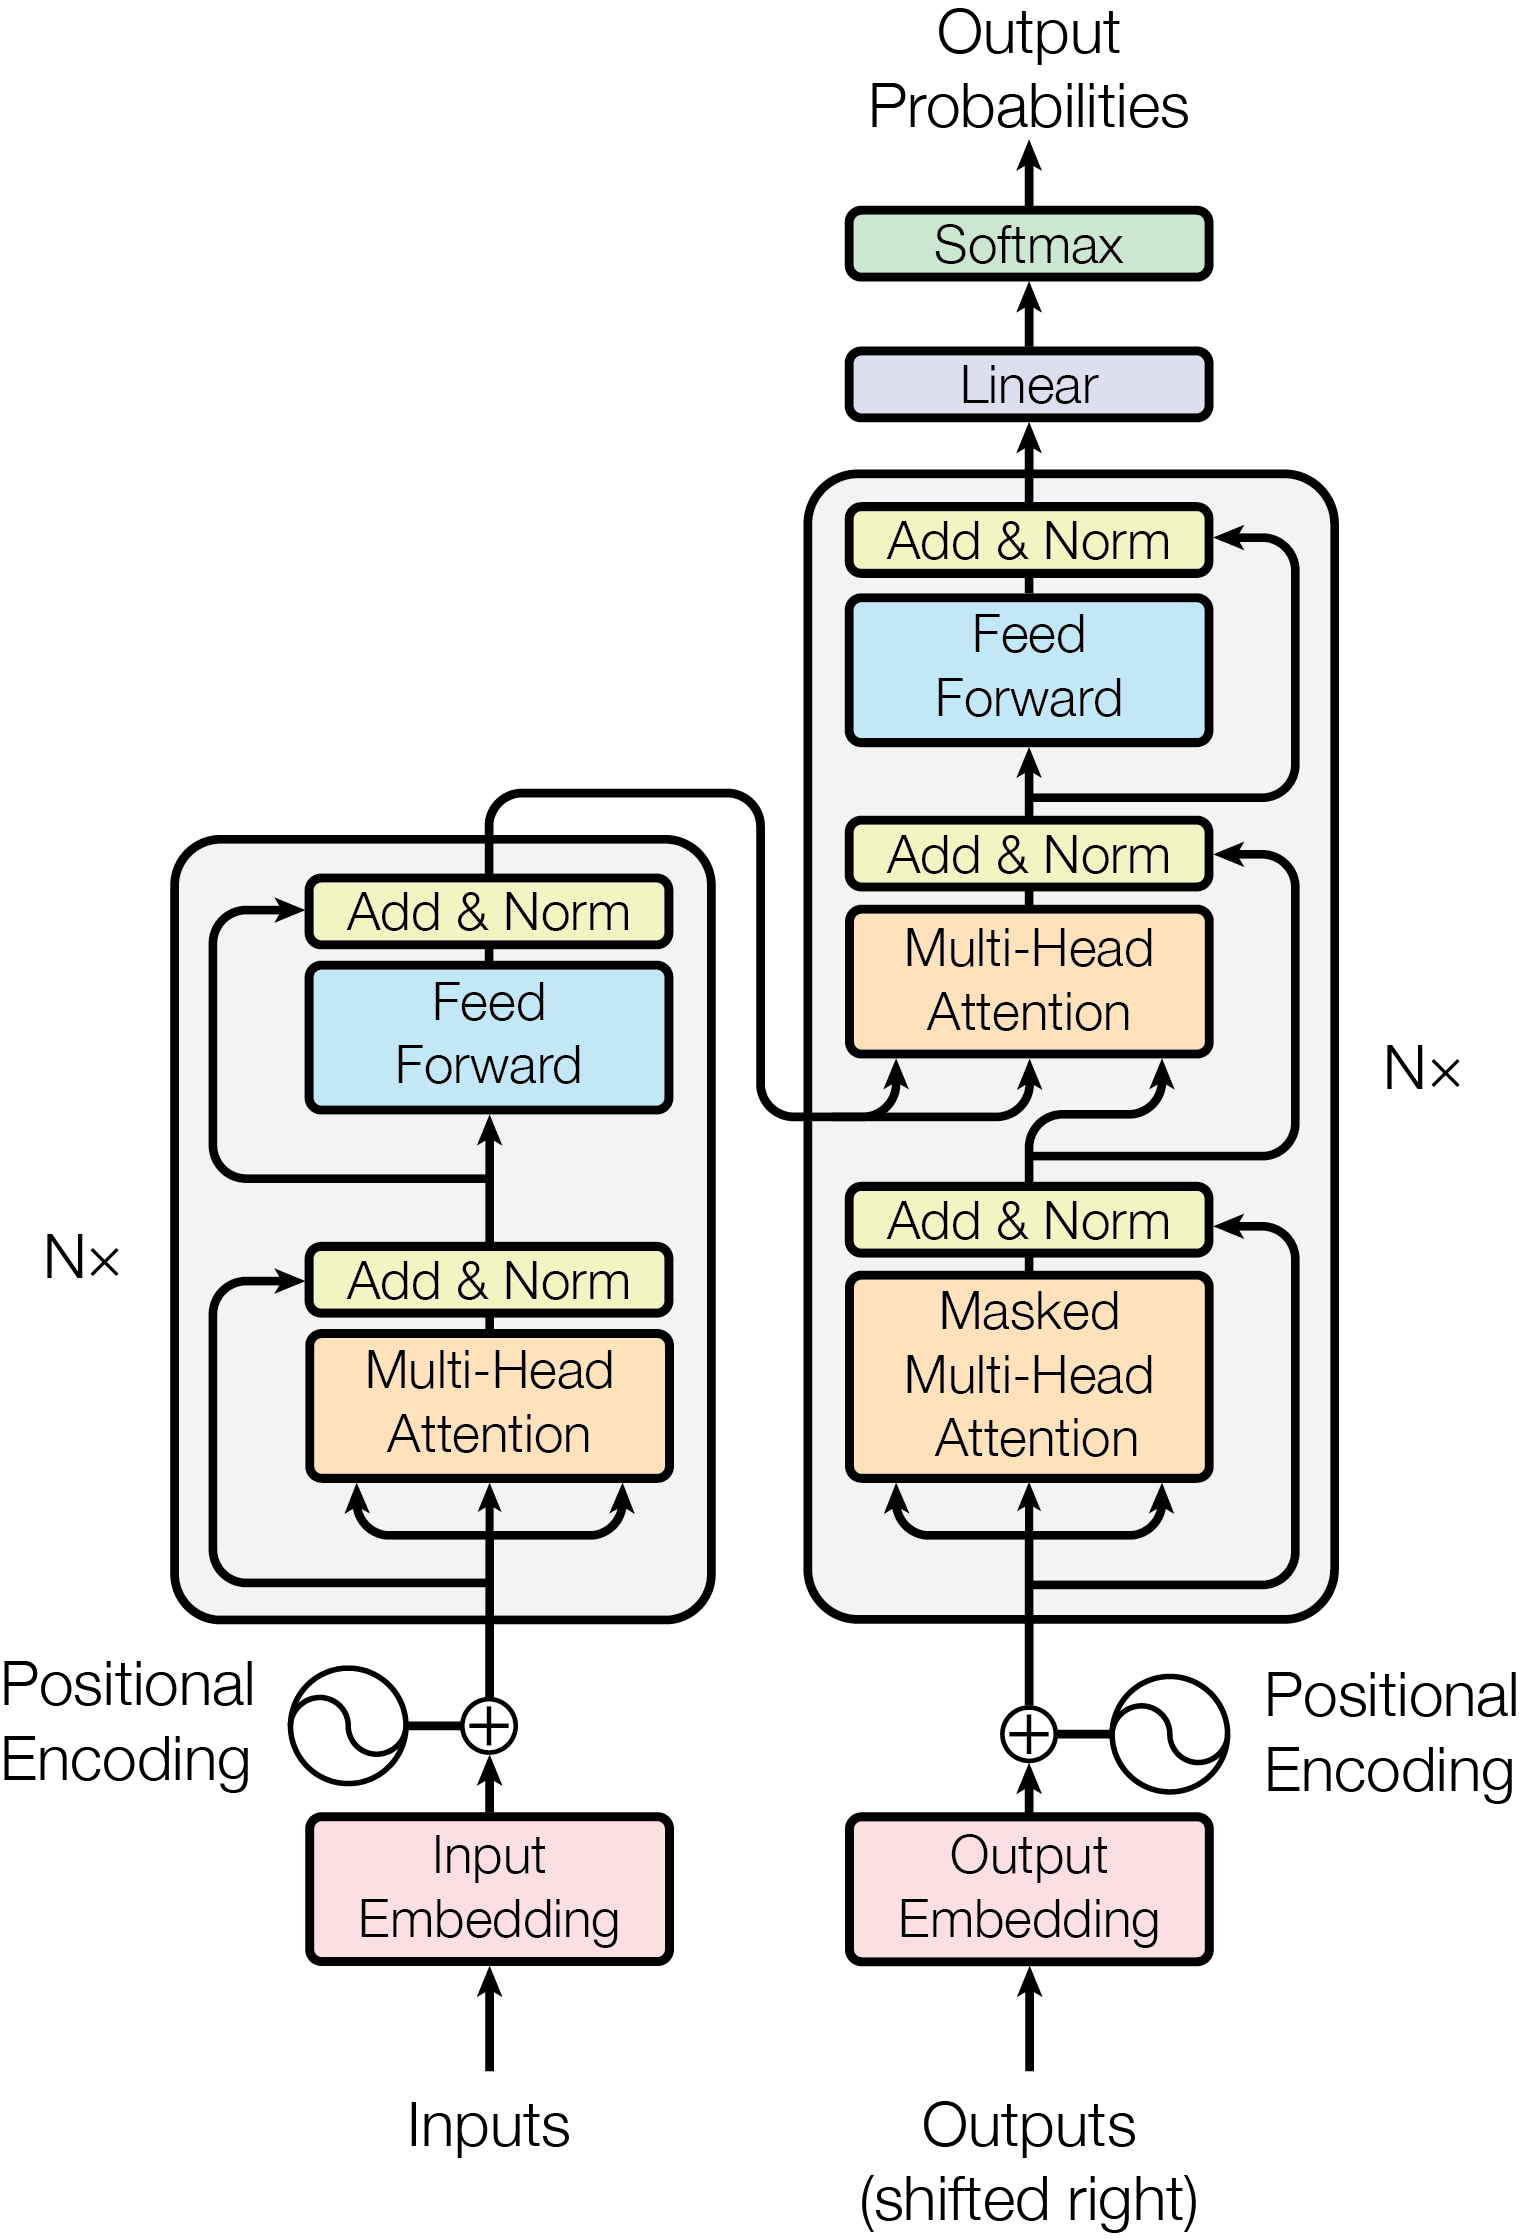
\includegraphics[scale=0.6]{Figures/ModalNet-21}
  \caption{The Transformer - model architecture.}
  \label{fig:model-arch}
\end{figure}

% Although the primary workhorse of our model is attention, 
%Our model maintains the encoder-decoder structure that is common to many so-called sequence-to-sequence models \citep{bahdanau2014neural,sutskever14}.  As in all such architectures, the encoder computes a representation of the input sequence, and the decoder consumes these representations along with the output tokens to autoregressively produce the output sequence.  Where, traditionally, the encoder and decoder contain stacks of recurrent or convolutional layers, our encoder and decoder stacks are composed of attention layers and position-wise feed-forward layers (Figure~\ref{fig:model-arch}).  The following sections describe the gross architecture and these particular components in detail.

Most competitive neural sequence transduction models have an encoder-decoder structure \citep{cho2014learning,bahdanau2014neural,sutskever14}. Here, the encoder maps an input sequence of symbol representations $(x_1, ..., x_n)$ to a sequence of continuous representations $\mathbf{z} = (z_1, ..., z_n)$. Given $\mathbf{z}$, the decoder then generates an output sequence $(y_1,...,y_m)$ of symbols one element at a time. At each step the model is auto-regressive \citep{graves2013generating}, consuming the previously generated symbols as additional input when generating the next.

The Transformer follows this overall architecture using stacked self-attention and point-wise, fully connected layers for both the encoder and decoder, shown in the left and right halves of Figure~\ref{fig:model-arch}, respectively.

\subsection{Encoder and Decoder Stacks}

\paragraph{Encoder:}The encoder is composed of a stack of $N=6$ identical layers. Each layer has two sub-layers. The first is a multi-head self-attention mechanism, and the second is a simple, position-wise fully connected feed-forward network.   We employ a residual connection \citep{he2016deep} around each of the two sub-layers, followed by layer normalization \cite{layernorm2016}.  That is, the output of each sub-layer is $\mathrm{LayerNorm}(x + \mathrm{Sublayer}(x))$, where $\mathrm{Sublayer}(x)$ is the function implemented by the sub-layer itself.  To facilitate these residual connections, all sub-layers in the model, as well as the embedding layers, produce outputs of dimension $\dmodel=512$.

\paragraph{Decoder:}The decoder is also composed of a stack of $N=6$ identical layers.  In addition to the two sub-layers in each encoder layer, the decoder inserts a third sub-layer, which performs multi-head attention over the output of the encoder stack.  Similar to the encoder, we employ residual connections around each of the sub-layers, followed by layer normalization.  We also modify the self-attention sub-layer in the decoder stack to prevent positions from attending to subsequent positions.  This masking, combined with fact that the output embeddings are offset by one position, ensures that the predictions for position $i$ can depend only on the known outputs at positions less than $i$.

% In our model (Figure~\ref{fig:model-arch}), the encoder and decoder are composed of stacks of alternating self-attention layers (for cross-positional communication) and position-wise feed-forward layers (for in-place computation).  In addition, the decoder stack contains encoder-decoder attention layers.  Since attention is agnostic to the distances between words, our model requires a "positional encoding" to be added to the encoder and decoder input. The following sections describe all of these components in detail.

\subsection{Attention} \label{sec:attention}
An attention function can be described as mapping a query and a set of key-value pairs to an output, where the query, keys, values, and output are all vectors.  The output is computed as a weighted sum of the values, where the weight assigned to each value is computed by a compatibility function of the query with the corresponding key.

\subsubsection{Scaled Dot-Product Attention} \label{sec:scaled-dot-prod}

% \begin{figure}
%   \centering
%   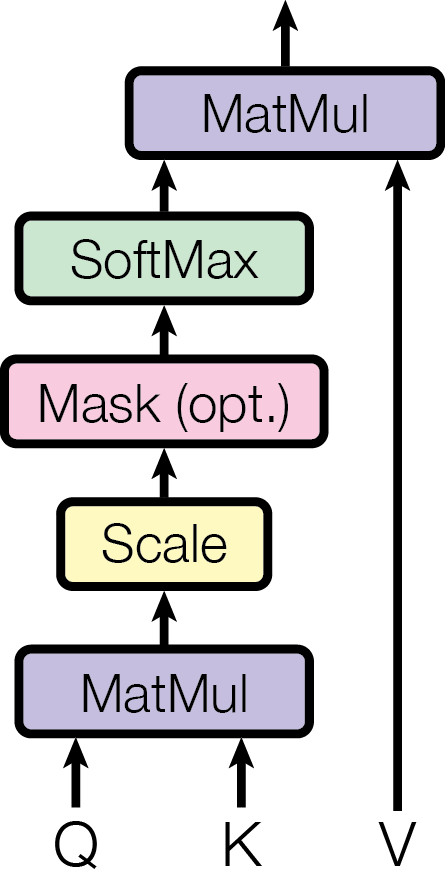
\includegraphics[scale=0.6]{Figures/ModalNet-19}
%   \caption{Scaled Dot-Product Attention.}
%   \label{fig:multi-head-att}
% \end{figure}

We call our particular attention "Scaled Dot-Product Attention" (Figure~\ref{fig:multi-head-att}).   The input consists of queries and keys of dimension $d_k$, and values of dimension $d_v$.  We compute the dot products of the query with all keys, divide each by $\sqrt{d_k}$, and apply a softmax function to obtain the weights on the values.

In practice, we compute the attention function on a set of queries simultaneously, packed together into a matrix $Q$.   The keys and values are also packed together into matrices $K$ and $V$.  We compute the matrix of outputs as:

\begin{equation}
   \mathrm{Attention}(Q, K, V) = \mathrm{softmax}(\frac{QK^T}{\sqrt{d_k}})V
\end{equation}

The two most commonly used attention functions are additive attention \citep{bahdanau2014neural}, and dot-product (multiplicative) attention.  Dot-product attention is identical to our algorithm, except for the scaling factor of $\frac{1}{\sqrt{d_k}}$. Additive attention computes the compatibility function using a feed-forward network with a single hidden layer.  While the two are similar in theoretical complexity, dot-product attention is much faster and more space-efficient in practice, since it can be implemented using highly optimized matrix multiplication code. 

%We scale the dot products by $1/\sqrt{d_k}$ to limit the magnitude of the dot products, which works well in practice. Otherwise, we found applying the softmax to often result in weights very close to 0 or 1, and hence minuscule gradients.

% Already described in the subsequent section
%When used as part of decoder self-attention, an optional mask function is applied just before the softmax to prevent positions from attending to subsequent positions.   This mask simply sets the logits corresponding to all illegal connections (those outside of the lower triangle) to $-\infty$.

%\paragraph{Comparison to Additive Attention: } We choose dot product attention over additive attention \citep{bahdanau2014neural} since it can be computed using highly optimized matrix multiplication code.  This optimization is particularly important to us, as we employ many attention layers in our model.

While for small values of $d_k$ the two mechanisms perform similarly, additive attention outperforms dot product attention without scaling for larger values of $d_k$ \citep{DBLP:journals/corr/BritzGLL17}. We suspect that for large values of $d_k$, the dot products grow large in magnitude, pushing the softmax function into regions where it has extremely small gradients  \footnote{To illustrate why the dot products get large, assume that the components of $q$ and $k$ are independent random variables with mean $0$ and variance $1$.  Then their dot product, $q \cdot k = \sum_{i=1}^{d_k} q_ik_i$, has mean $0$ and variance $d_k$.}. To counteract this effect, we scale the dot products by $\frac{1}{\sqrt{d_k}}$.


%We suspect this to be caused by the dot products growing too large in magnitude to result in useful gradients after applying the softmax function.  To counteract this, we scale the dot product by $1/\sqrt{d_k}$.


\subsubsection{Multi-Head Attention} \label{sec:multihead}

\begin{figure}
\begin{minipage}[t]{0.5\textwidth}
  \centering
  Scaled Dot-Product Attention \\
  \vspace{0.5cm}
  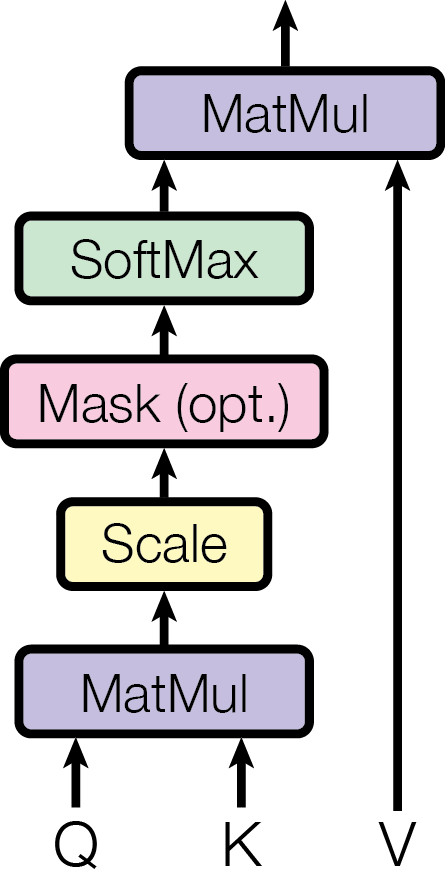
\includegraphics[scale=0.6]{Figures/ModalNet-19}
\end{minipage}
\begin{minipage}[t]{0.5\textwidth}
  \centering 
  Multi-Head Attention \\
  \vspace{0.1cm}
  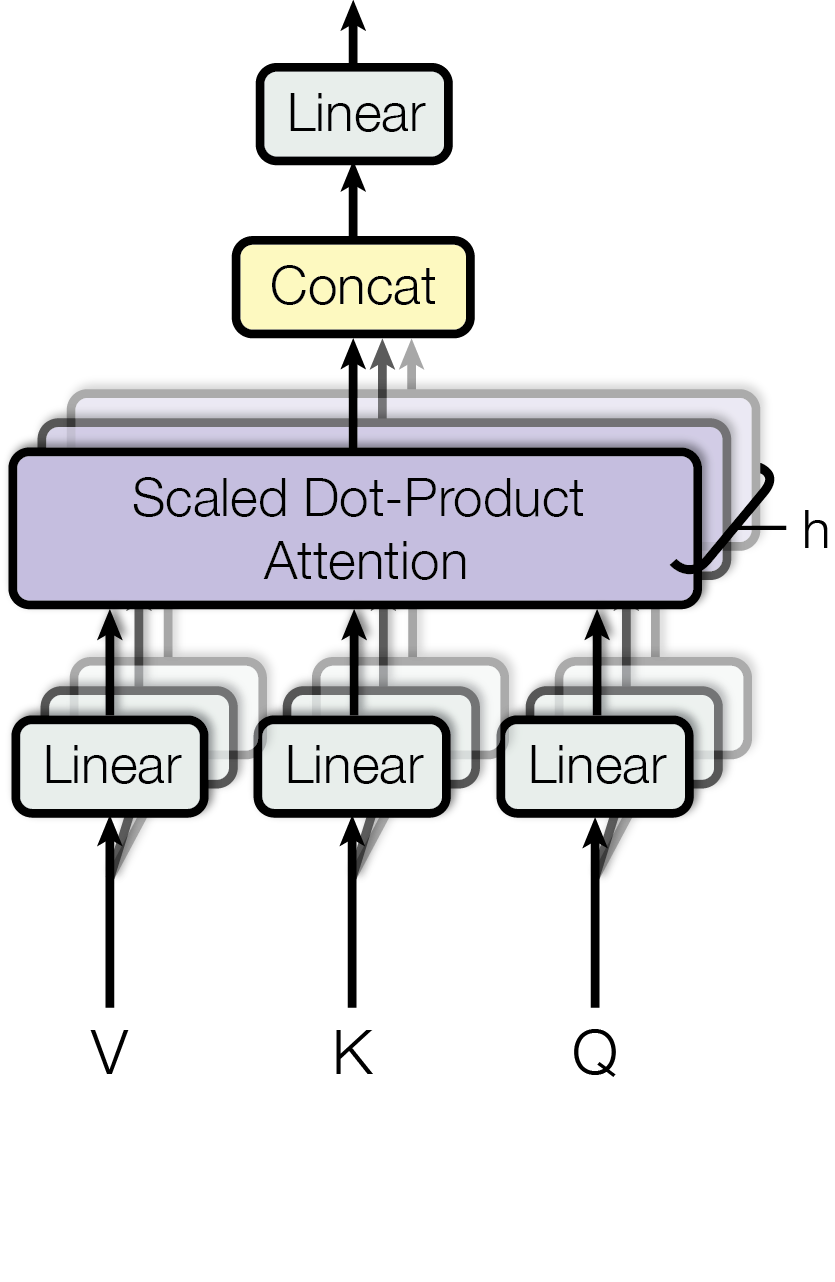
\includegraphics[scale=0.6]{Figures/ModalNet-20}  
\end{minipage}


  % \centering

  \caption{(left) Scaled Dot-Product Attention. (right) Multi-Head Attention consists of several attention layers running in parallel.}
  \label{fig:multi-head-att}
\end{figure}

Instead of performing a single attention function with $\dmodel$-dimensional keys, values and queries, we found it beneficial to linearly project the queries, keys and values $h$ times with different, learned linear projections to $d_k$, $d_k$ and $d_v$ dimensions, respectively.
On each of these projected versions of queries, keys and values we then perform the attention function in parallel, yielding $d_v$-dimensional output values. These are concatenated and once again projected, resulting in the final values, as depicted in Figure~\ref{fig:multi-head-att}.

Multi-head attention allows the model to jointly attend to information from different representation subspaces at different positions. With a single attention head, averaging inhibits this.

\begin{align*}
    \mathrm{MultiHead}(Q, K, V) &= \mathrm{Concat}(\mathrm{head_1}, ..., \mathrm{head_h})W^O\\
%    \mathrm{where} \mathrm{head_i} &= \mathrm{Attention}(QW_Q_i^{\dmodel \times d_q}, KW_K_i^{\dmodel \times d_k}, VW^V_i^{\dmodel \times d_v})\\
    \text{where}~\mathrm{head_i} &= \mathrm{Attention}(QW^Q_i, KW^K_i, VW^V_i)\\
\end{align*}

Where the projections are parameter matrices $W^Q_i \in \mathbb{R}^{\dmodel \times d_k}$, $W^K_i \in \mathbb{R}^{\dmodel \times d_k}$, $W^V_i \in \mathbb{R}^{\dmodel \times d_v}$ and $W^O \in \mathbb{R}^{hd_v \times \dmodel}$.


%find it better (and no more expensive) to have multiple parallel attention layers (each over the full set of positions) with proportionally lower-dimensional keys, values and queries.  We call this "Multi-Head Attention" (Figure~\ref{fig:multi-head-att}).  The keys, values, and queries for each of these parallel attention layers are computed by learned linear transformations of the inputs to the multi-head attention.  We use different linear transformations across different parallel attention layers.  The output of the parallel attention layers are concatenated, and then passed through a final learned linear transformation. 

In this work we employ $h=8$ parallel attention layers, or heads. For each of these we use $d_k=d_v=\dmodel/h=64$.
Due to the reduced dimension of each head, the total computational cost is similar to that of single-head attention with full dimensionality.

\subsubsection{Applications of Attention in our Model}

The Transformer uses multi-head attention in three different ways: 
\begin{itemize}
 \item In "encoder-decoder attention" layers, the queries come from the previous decoder layer, and the memory keys and values come from the output of the encoder.   This allows every position in the decoder to attend over all positions in the input sequence.  This mimics the typical encoder-decoder attention mechanisms in sequence-to-sequence models such as \citep{wu2016google, bahdanau2014neural,JonasFaceNet2017}.

 \item The encoder contains self-attention layers.  In a self-attention layer all of the keys, values and queries come from the same place, in this case, the output of the previous layer in the encoder.   Each position in the encoder can attend to all positions in the previous layer of the encoder.

 \item Similarly, self-attention layers in the decoder allow each position in the decoder to attend to all positions in the decoder up to and including that position.  We need to prevent leftward information flow in the decoder to preserve the auto-regressive property.  We implement this inside of scaled dot-product attention by masking out (setting to $-\infty$) all values in the input of the softmax which correspond to illegal connections.  See Figure~\ref{fig:multi-head-att}.

\end{itemize}

\subsection{Position-wise Feed-Forward Networks}\label{sec:ffn}

In addition to attention sub-layers, each of the layers in our encoder and decoder contains a fully connected feed-forward network, which is applied to each position separately and identically.  This consists of two linear transformations with a ReLU activation in between.

\begin{equation}
   \mathrm{FFN}(x)=\max(0, xW_1 + b_1) W_2 + b_2
\end{equation}

While the linear transformations are the same across different positions, they use different parameters from layer to layer. Another way of describing this is as two convolutions with kernel size 1.  The dimensionality of input and output is $\dmodel=512$, and the inner-layer has dimensionality $d_{ff}=2048$.



%In the appendix, we describe how the position-wise feed-forward network can also be seen as a form of attention.

%from Jakob: The number of operations required for the model to relate signals from two arbitrary input or output positions grows in the distance between positions in input or output, linearly for ConvS2S and logarithmically for ByteNet, making it harder to learn dependencies between these positions \citep{hochreiter2001gradient}. In the transformer this is reduced to a constant number of operations, albeit at the cost of effective resolution caused by averaging attention-weighted positions, an effect we aim to counteract with multi-headed attention.


%Figure~\ref{fig:simple-att} presents a simple attention function, $A$, with a single head, that forms the basis of our multi-head attention. $A$ takes a query key vector $\kq$, matrices of memory keys $\km$ and memory values $\vm$ ,and produces a query value vector $\vq$ as 
%\begin{equation*} \label{eq:attention}
%    A(\kq, \km, \vm) = {\vm}^T (Softmax(\km \kq).
%\end{equation*}
%We linearly transform $\kq,\,\km$, and $\vm$ with learned matrices ${\Wkq \text{,} \, \Wkm}$, and ${\Wvm}$ before calling the attention function, and transform the output query with $\Wvq$ before handing it to the feed forward layer. Each attention layer has it's own set of transformation matrices, which are shared across all query positions. $A$ is applied in parallel for each query position, and is implemented very efficiently as a batch of matrix multiplies. The self-attention and encoder-decoder attention layers use $A$, but with different arguments. For example, in encdoder self-attention, queries in encoder layer $i$ attention to memories in encoder layer $i-1$. To ensure that decoder self-attention layers do not look at future words, we add $- \inf$ to the softmax logits in positions $j+1$ to query length for query position $l$.  

%In simple attention, the query value is a weighted combination of the memory values where the attention weights sum to one. Although this function performs well in practice, the constraint on attention weights can restrict the amount of information that flows from memories to queries because the query cannot focus on multiple memory positions at once, which might be desirable when translating long sequences. \marginpar{@usz, could you think of an example of this ?} We remedy this by maintaining multiple attention heads at each query position that attend to all memory positions in parallel, with a different set of parameters  per attention head $h$. 
%\marginpar{}

\subsection{Embeddings and Softmax}
Similarly to other sequence transduction models, we use learned embeddings to convert the input tokens and output tokens to vectors of dimension $\dmodel$.  We also use the usual learned linear transformation and softmax function to convert the decoder output to predicted next-token probabilities.  In our model, we share the same weight matrix between the two embedding layers and the pre-softmax linear transformation, similar to \citep{press2016using}.   In the embedding layers, we multiply those weights by $\sqrt{\dmodel}$.


\subsection{Positional Encoding}
Since our model contains no recurrence and no convolution, in order for the model to make use of the order of the sequence, we must inject some information about the relative or absolute position of the tokens in the sequence.  To this end, we add "positional encodings" to the input embeddings at the bottoms of the encoder and decoder stacks.  The positional encodings have the same dimension $\dmodel$ as the embeddings, so that the two can be summed.   There are many choices of positional encodings, learned and fixed \citep{JonasFaceNet2017}.

In this work, we use sine and cosine functions of different frequencies:

\begin{align*}
    PE_{(pos,2i)} = sin(pos / 10000^{2i/\dmodel}) \\
    PE_{(pos,2i+1)} = cos(pos / 10000^{2i/\dmodel})
\end{align*}

where $pos$ is the position and $i$ is the dimension.  That is, each dimension of the positional encoding corresponds to a sinusoid.  The wavelengths form a geometric progression from $2\pi$ to $10000 \cdot 2\pi$.  We chose this function because we hypothesized it would allow the model to easily learn to attend by relative positions, since for any fixed offset $k$, $PE_{pos+k}$ can be represented as a linear function of $PE_{pos}$.

We also experimented with using learned positional embeddings \citep{JonasFaceNet2017} instead, and found that the two versions produced nearly identical results (see Table~\ref{tab:variations} row (E)).  We chose the sinusoidal version because it may allow the model to extrapolate to sequence lengths longer than the ones encountered during training.
